%%
% Plantilla de Presentación
% Modificación de una plantilla de Latex de LaTeXTemplates para adaptarla 
% al castellano y a las necesidades de escribir informática y matemáticas.
%
% Editada por: Mario Román
%
% License:
% CC BY-NC-SA 3.0 (http://creativecommons.org/licenses/by-nc-sa/3.0/)
%%

%%%%%%%%%%%%%%%%%%%%%
% Beamer Presentation
% LaTeX Template
% Version 1.0 (10/11/12)
%
% This template has been downloaded from:
% http://www.LaTeXTemplates.com
%
% License:
% CC BY-NC-SA 3.0 (http://creativecommons.org/licenses/by-nc-sa/3.0/)
%
%%%%%%%%%%%%%%%%%%%%%

%----------------------------------------------------------------------------------------
%	PAQUETES Y CONFIGURACIÓN DEL DOCUMENTO
%----------------------------------------------------------------------------------------

\documentclass[compress, aspectratio=169]{beamer} % Beamer
\usepackage[spanish]{babel} % Traducciones
\usepackage[utf8]{inputenc} % Uso de caracteres UTF-8
\usepackage[T1]{fontenc} % Permite copiar código y evita errores
\uselanguage{Spanish} % Traducciones beamer
\languagepath{Spanish} % (tex.stackexchange.com/questions/168208)
\usepackage{pgfpages} % Beamer User Guide sections 19.6 and 22
\usepackage[absolute,overlay]{textpos} % Especifica posición del texto.
\usepackage{verbatim} % Bloques de comentarios

%% Temas %%
% Tema y tema de color
\usetheme{CambridgeUS}
\usecolortheme{beaver}

% Fuentes de tamaño arbitrario
\usepackage{lmodern}

% Gráficos
\usepackage{graphicx} % Allows including images
\usepackage{booktabs} % Allows the use of \toprule, \midrule and \bottomrule in tables

%----------------------------------------------------------------------------------------
%	TÍTULO
%----------------------------------------------------------------------------------------

%% Título y otros %%
\title[smart-plug]{Diseño y construcción de un sistema para adquisición y análisis del consumo energético en el hogar} % The short title appears at the bottom of every slide, the full title is only on the title page

\author[Jesús Sánchez de Lechina Tejada]{
	Jesús Sánchez de Lechina Tejada
	(\href{http://www.github.com/jojelupipa}{@jojelupipa})\\ 
} % Your name

\institute[UGR] % Your institution as it will appear on the bottom of every slide, may be shorthand to save space
{
  Universidad de Granada \\ % Your institution for the title page
}
\date{Julio 2020} % Date, can be changed to a custom date

\begin{document}

% Diapositiva de título.
\begin{frame}
	\transdissolve[duration=1]

	\titlepage % Print the title page as the first slide
        \centering 
\includegraphics[scale=0.3]{img/by.png}
\end{frame}


%----------------------------------------------------------------------------------------
%	PRESENTACIÓN
%----------------------------------------------------------------------------------------
 
%------------------------------------------------
\begin{frame}
  \transdissolve[duration=1]
  \tableofcontents[]
  \frametitle{Índice}
\end{frame}


\section{Introducción}
	\begin{frame}
	  \transdissolve[duration=1]
          \tableofcontents[currentsection,currentsubsection]
	  \frametitle{\insertsection}
	\end{frame}

        \begin{frame}
          \transdissolve[duration=1]
          \frametitle{¿Qué he hecho?}

          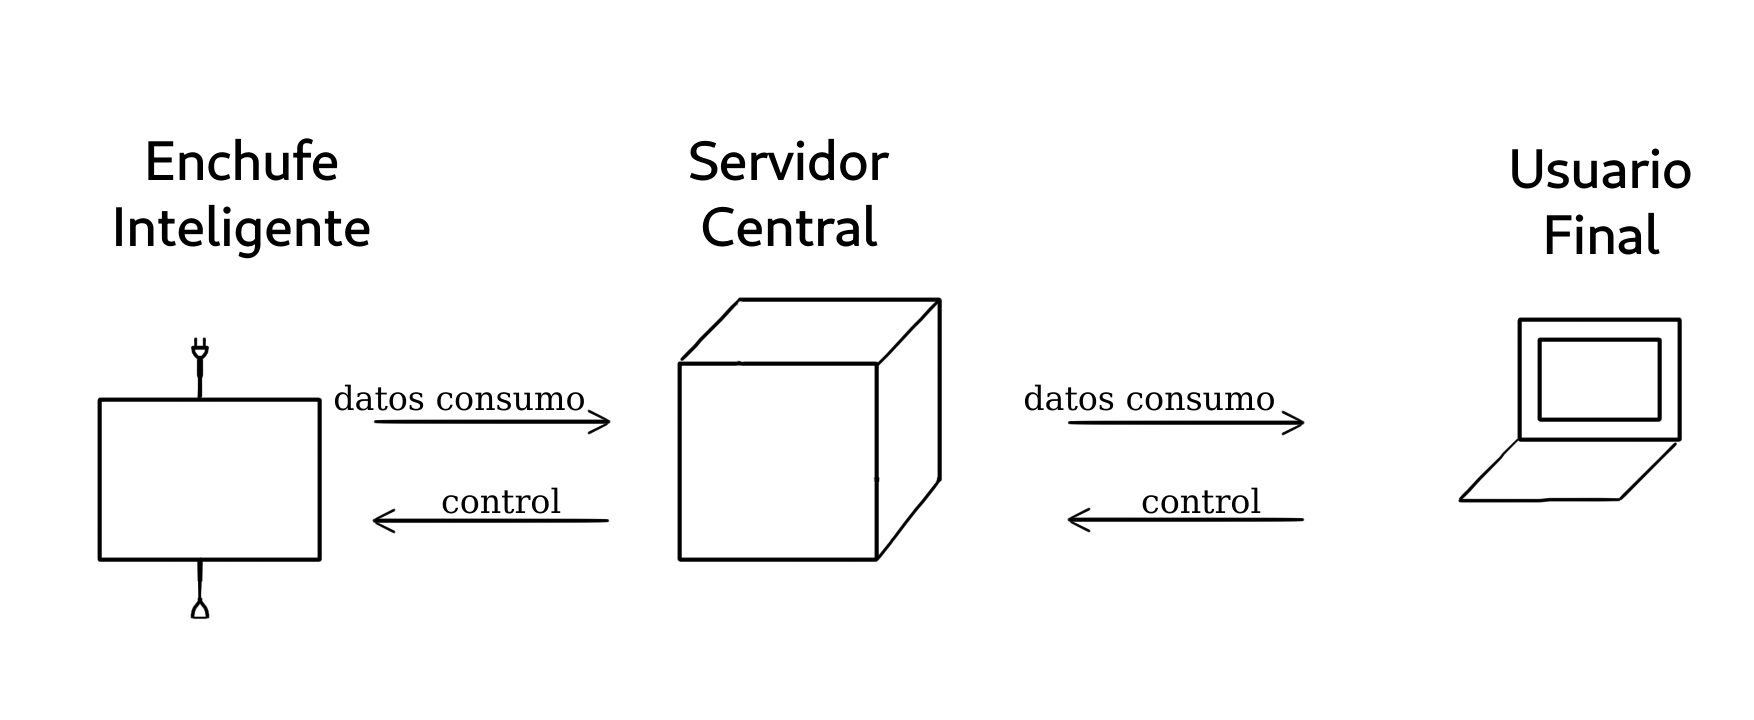
\includegraphics{img/esquema_basico_sistema.png}
          
          % En este TFG se ha diseñado y construido un sistema para
          % monitorizar el consumo en el hogar. Esto lo se ha hecho
          % mediante la construcción de un enchufe inteligente que
          % capte y transmita el consumo de un dispositivo enchufado
          % en corriente alterna, un medio donde almacenar esta info y
          % un medio en el que consultarla.
          %
          % Además se le ha añadido la utilidad de controlar el
          % encendido y apagado del dispositivo conectado mediante el
          % uso de un relé manejado por una señal enviada por el
          % usuario final.
          
        \end{frame}

        \begin{frame}
          \transdissolve[duration=1]
          \frametitle{Objetivos}

          \begin{itemize}
            \item{\only<1->{Construir un sistema para medir y controlar el
              consumo energético.}
            
            \uncover<2->{Para ello se utilizará una infraestructura y paradigma que
              se ajuste a este proyecto: \textit{Internet de las Cosas}.}}

            \item{\uncover<3->{Demostrar que el Internet de las Cosas
                está al alcance de cualquiera. Este proyecto es un
                ejemplo de ello.}}

          \end{itemize}

        \end{frame}
\section{Descripción del sistema}

\begin{frame}
  \transdissolve[duration=1]
  \frametitle{\insertsection}
  \tableofcontents[currentsection]

  % En esta sección se presenta una descripción de cada uno de los
  % elementos principales que componen el sistema, cómo se comunican y
  % una breve descripción sobre las pruebas que se han realizado.
\end{frame}

\subsection{Topología de red}
\begin{frame}
  \transdissolve[duration=1]
  \tableofcontents[currentsection,currentsubsection]
  \frametitle{\insertsubsection}
\end{frame}

\begin{frame}
  \transdissolve[duration=1]
  \frametitle{\insertsubsection}
  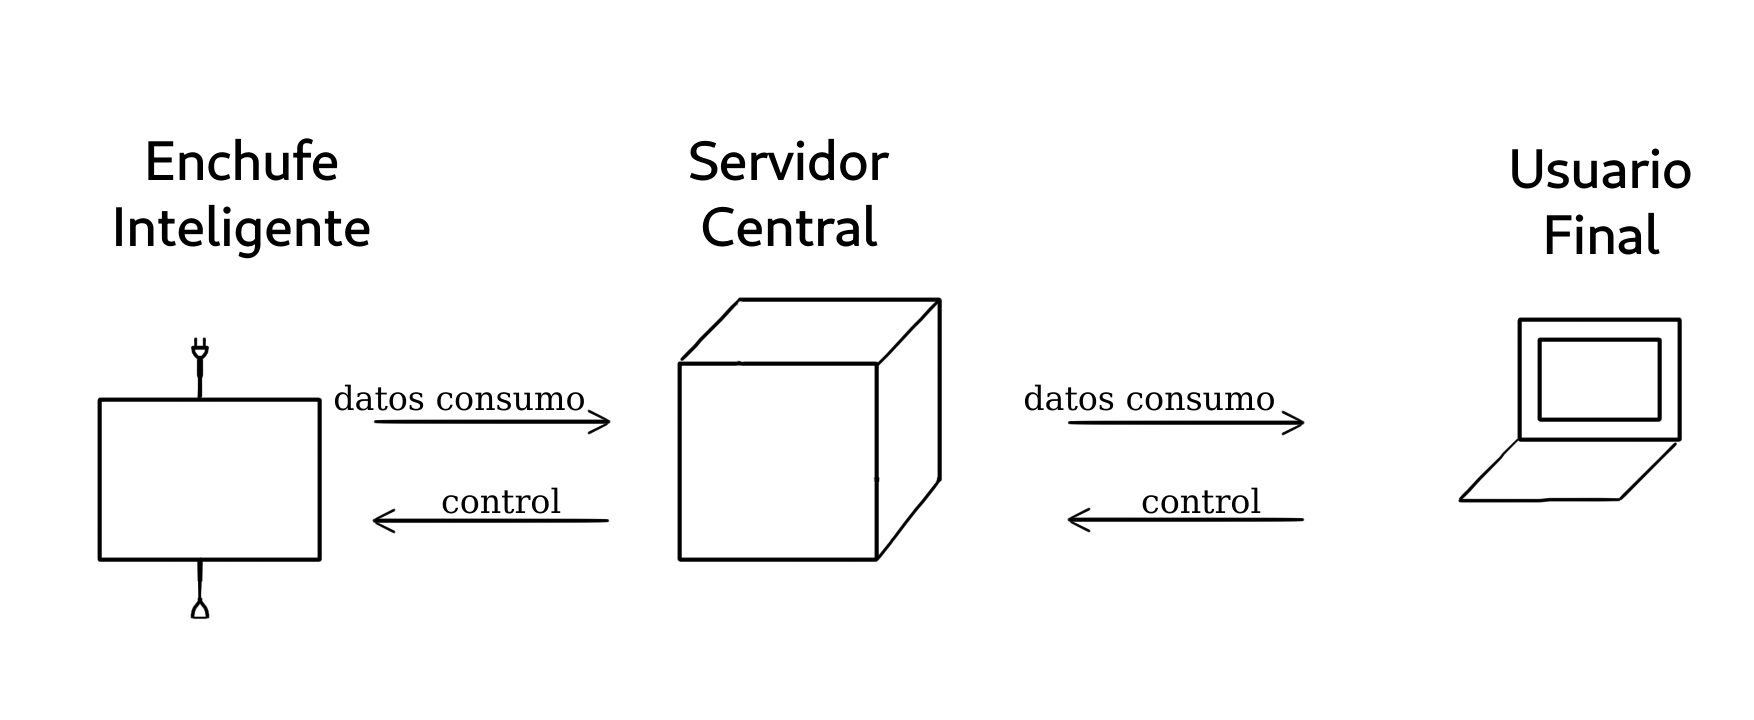
\includegraphics{img/esquema_basico_sistema.png}
  % Previamente mostrábamos este esquema del sistema, no es
  % completamente preciso pero nos sirve para conocer cada tipo de
  % nodo que hay en el sistema
\end{frame}

\begin{frame}
  \transdissolve[duration=1]
  \frametitle{\insertsubsection}
  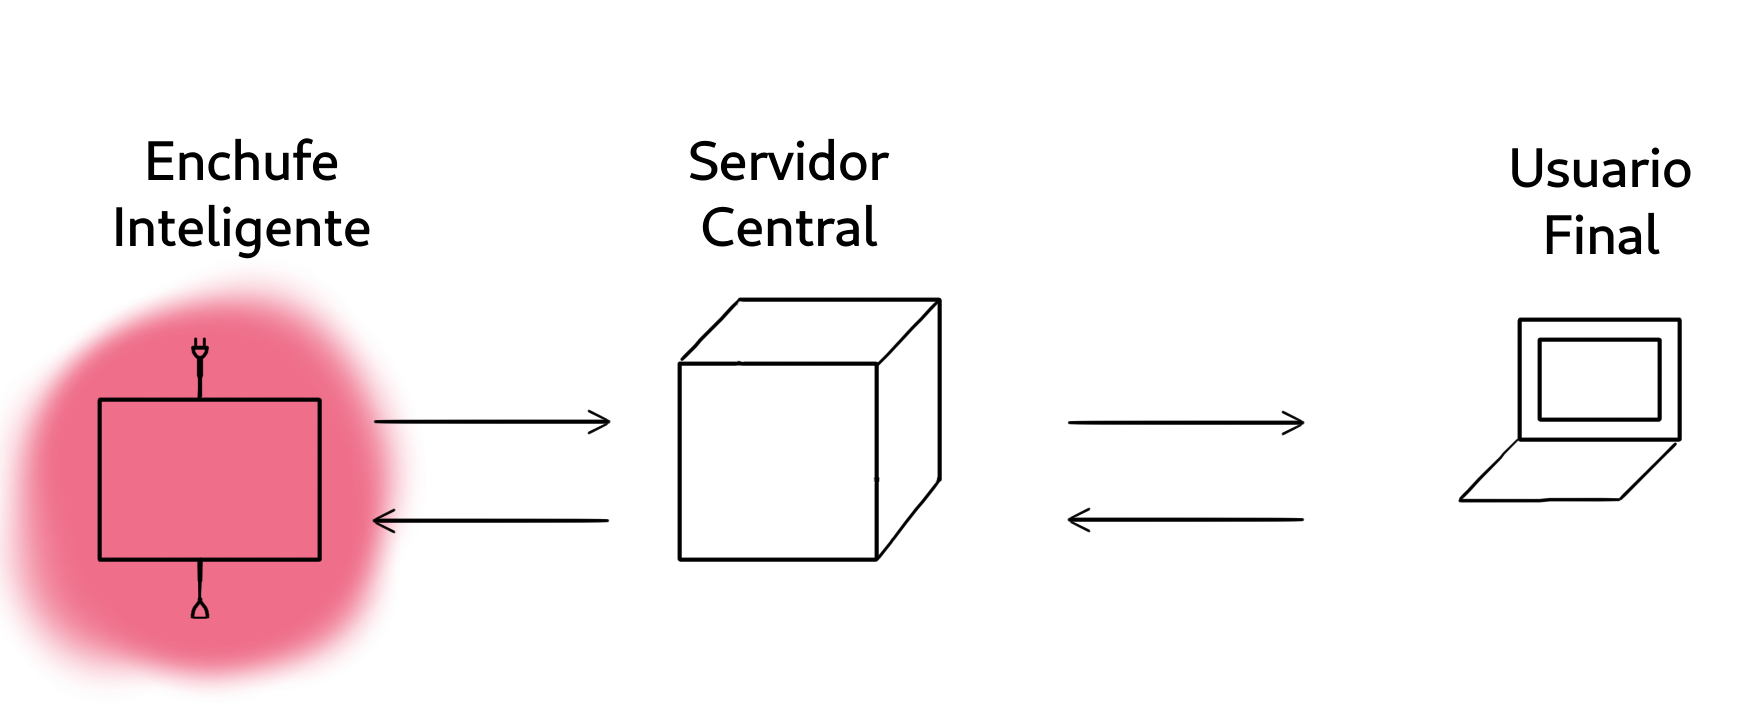
\includegraphics{img/esquema_basico_sistema_enchufe_resaltado.png}
  % El primer tipo de nodo es el enchufe inteligente, encargado de
  % medir el consumo de un enchufe y retransmitirlo al
  % servidor así como su manipulación. Pueden existir múltiples instancias.
\end{frame}

\begin{frame}
  \transdissolve[duration=1]
  \frametitle{\insertsubsection}
  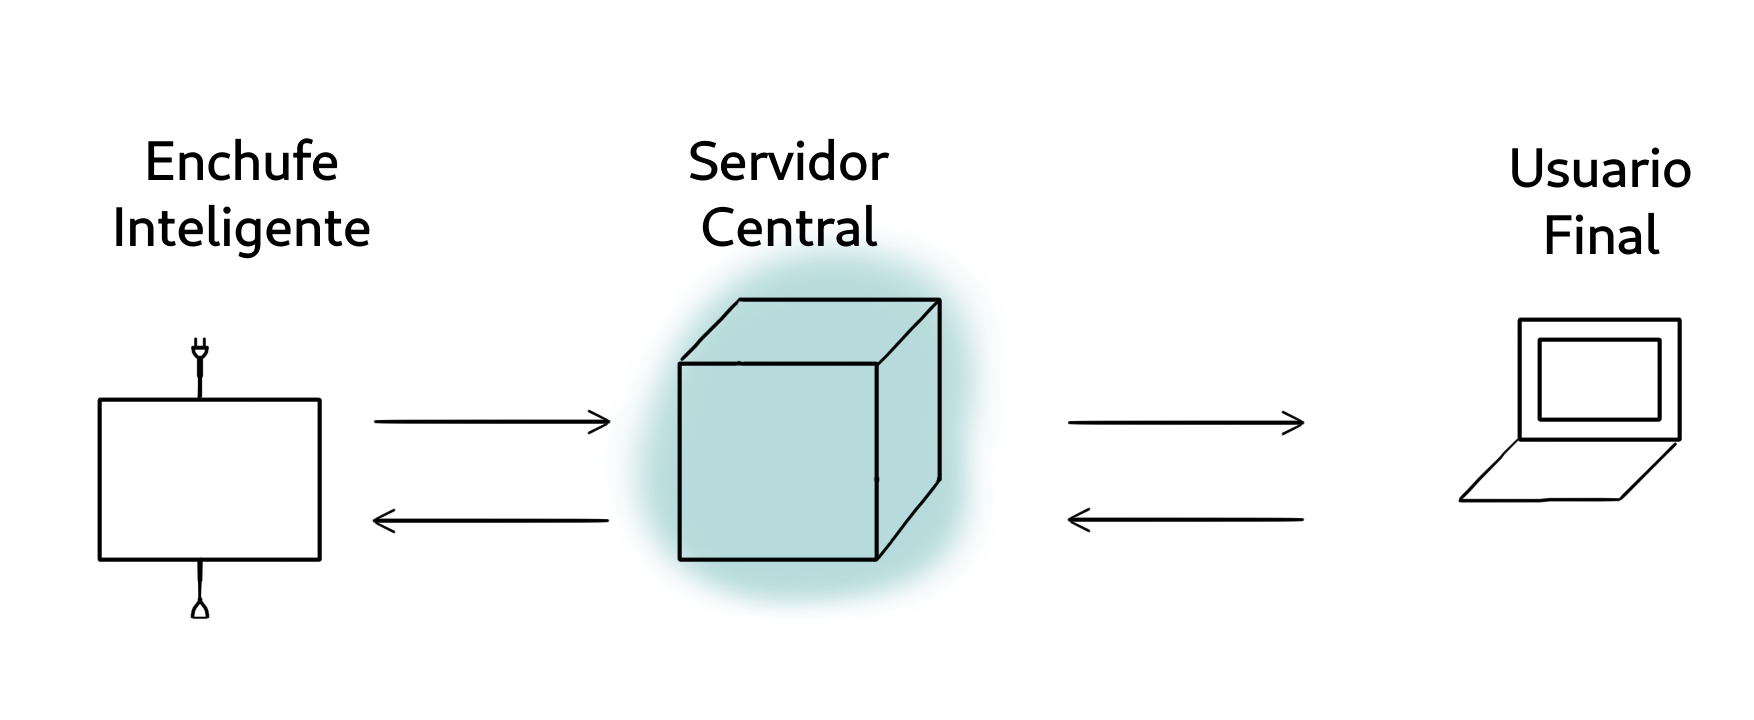
\includegraphics{img/esquema_basico_sistema_servidor_resaltado.png}
  % El segundo tipo de nodo es el servidor, encargado de almacenar la
  % información y de proporcionarla al usuario final. Existe una única
  % instancia.
\end{frame}

\begin{frame}
  \transdissolve[duration=1]
  \frametitle{\insertsubsection}
  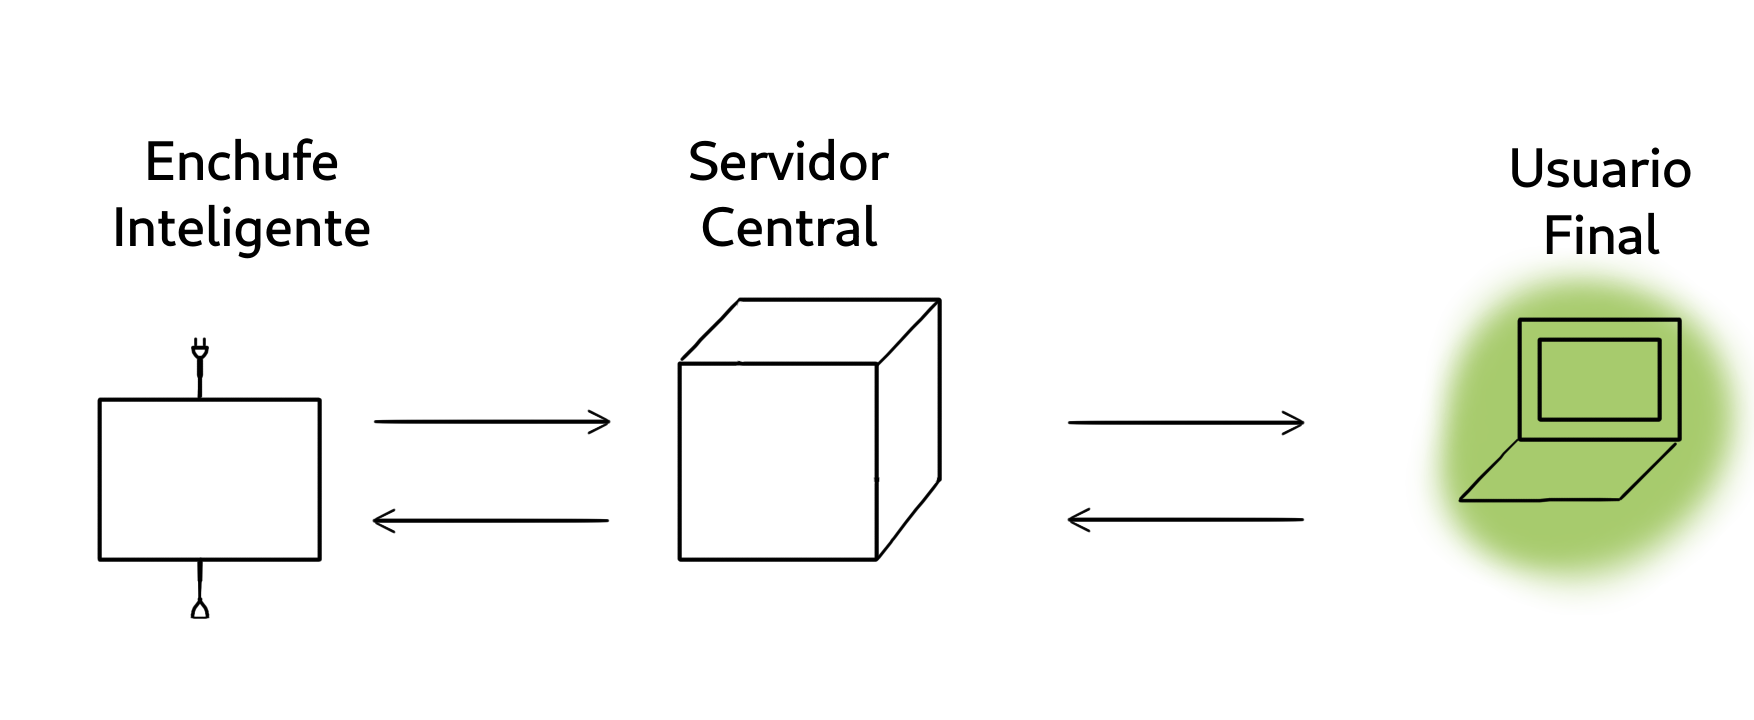
\includegraphics{img/esquema_basico_sistema_app_resaltado.png}
  % El último tipo de nodo es la aplicación final, encargado presentar
  % el consumo y enviar las órdenes de gestión a los enchufes. Pueden
  % existir múltiples instancias.
\end{frame}

\begin{frame}
  \transdissolve[duration=1]
  \frametitle{\insertsubsection}
  \centering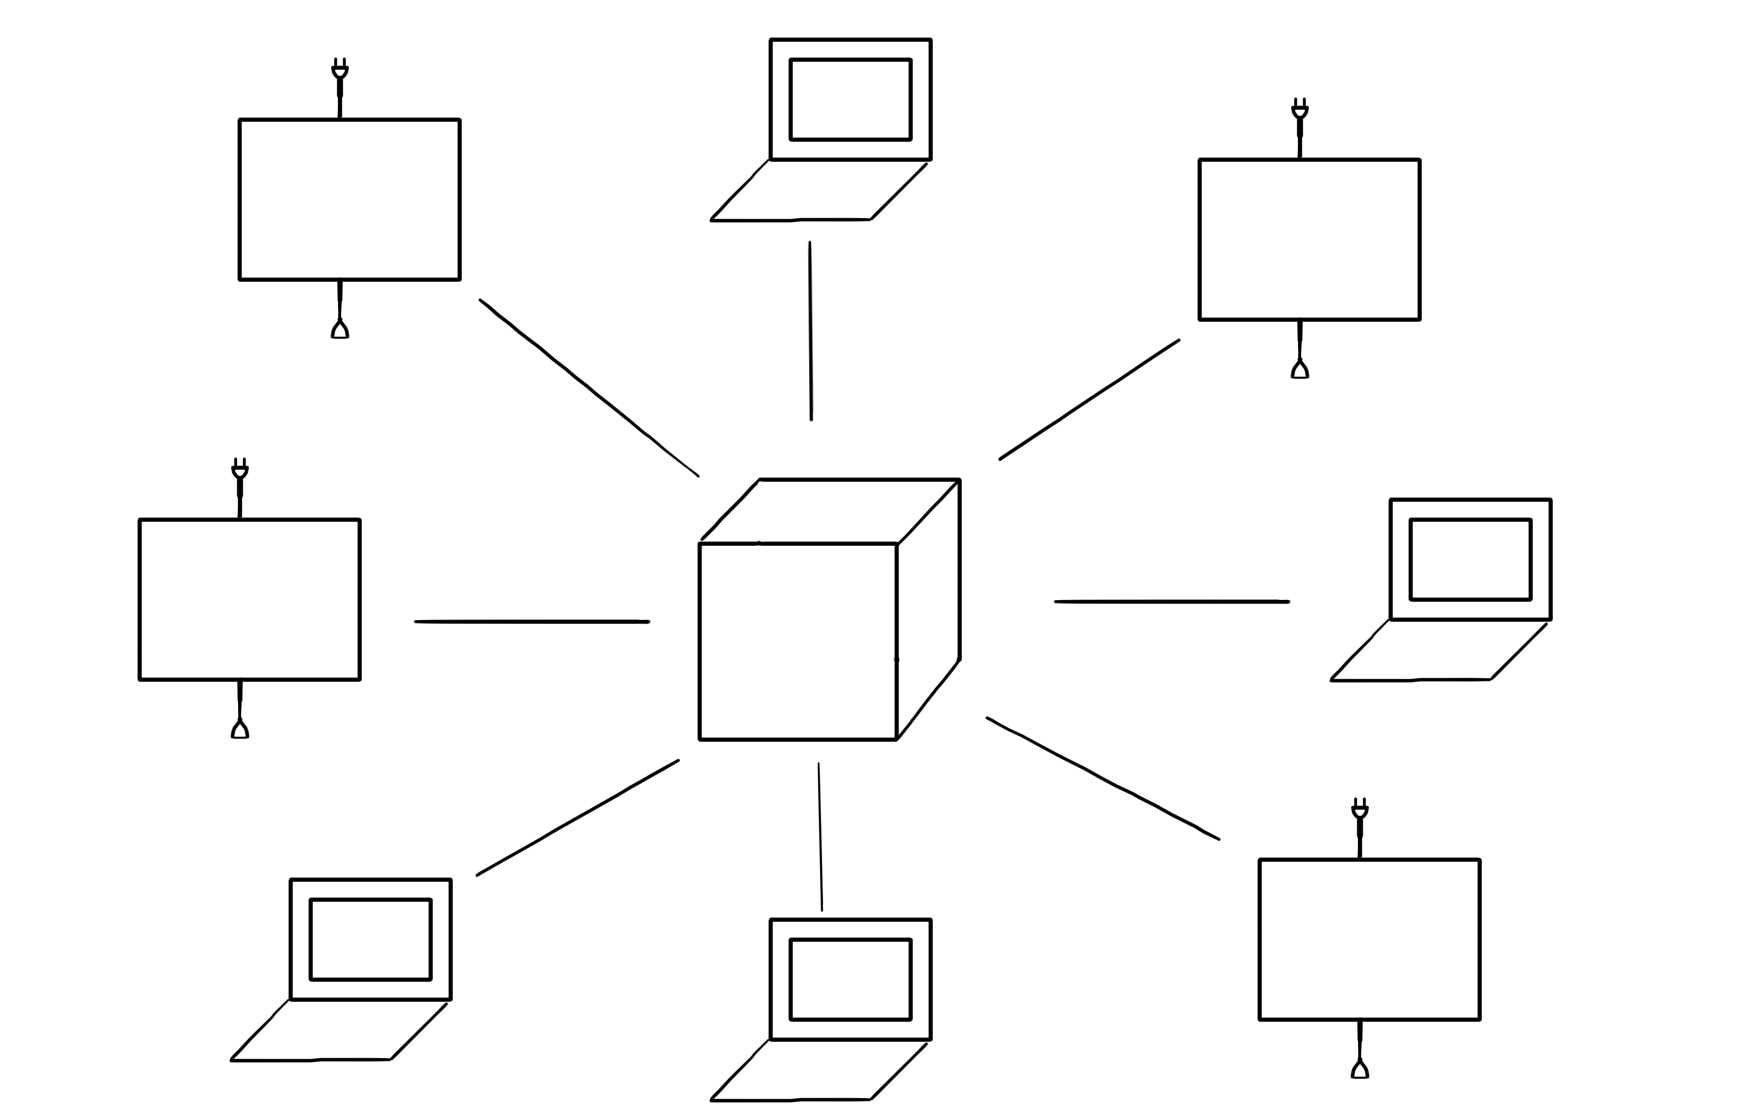
\includegraphics[scale=0.7]{img/esquema_estrella.png}
  % Esta representación refleja mejor la topología que se utiliza en
  % el sistema: Una topología de estrella en la que el servidor
  % central gestiona todas las comunicaciones y es el núcleo del
  % sistema y existen múltiples enchufes y usuarios que se conectan a
  % este.
\end{frame}

\begin{frame}
  \transdissolve[duration=1]
  \frametitle{\insertsubsection}
  ¿Cómo se comunican?
  \begin{itemize}
    \item{Control de enchufes: Mensajes MQTT gestionados por un Broker
      en el Servidor}
    \item{Datos Enchufe $\rightarrow$ Servidor: MQTT}
    \item{Datos Servidor $\rightarrow$ Cliente: Peticiones HTTP a
      una API}
  \end{itemize}
\end{frame}


\subsection{Módulo Enchufe Inteligente}
\begin{frame}
  \transdissolve[duration=1]
  \frametitle{\insertsubsection}
  \tableofcontents[currentsection,currentsubsection]
\end{frame}

\begin{frame}
  \transdissolve[duration=1]
  \frametitle{\insertsubsection}
  \centering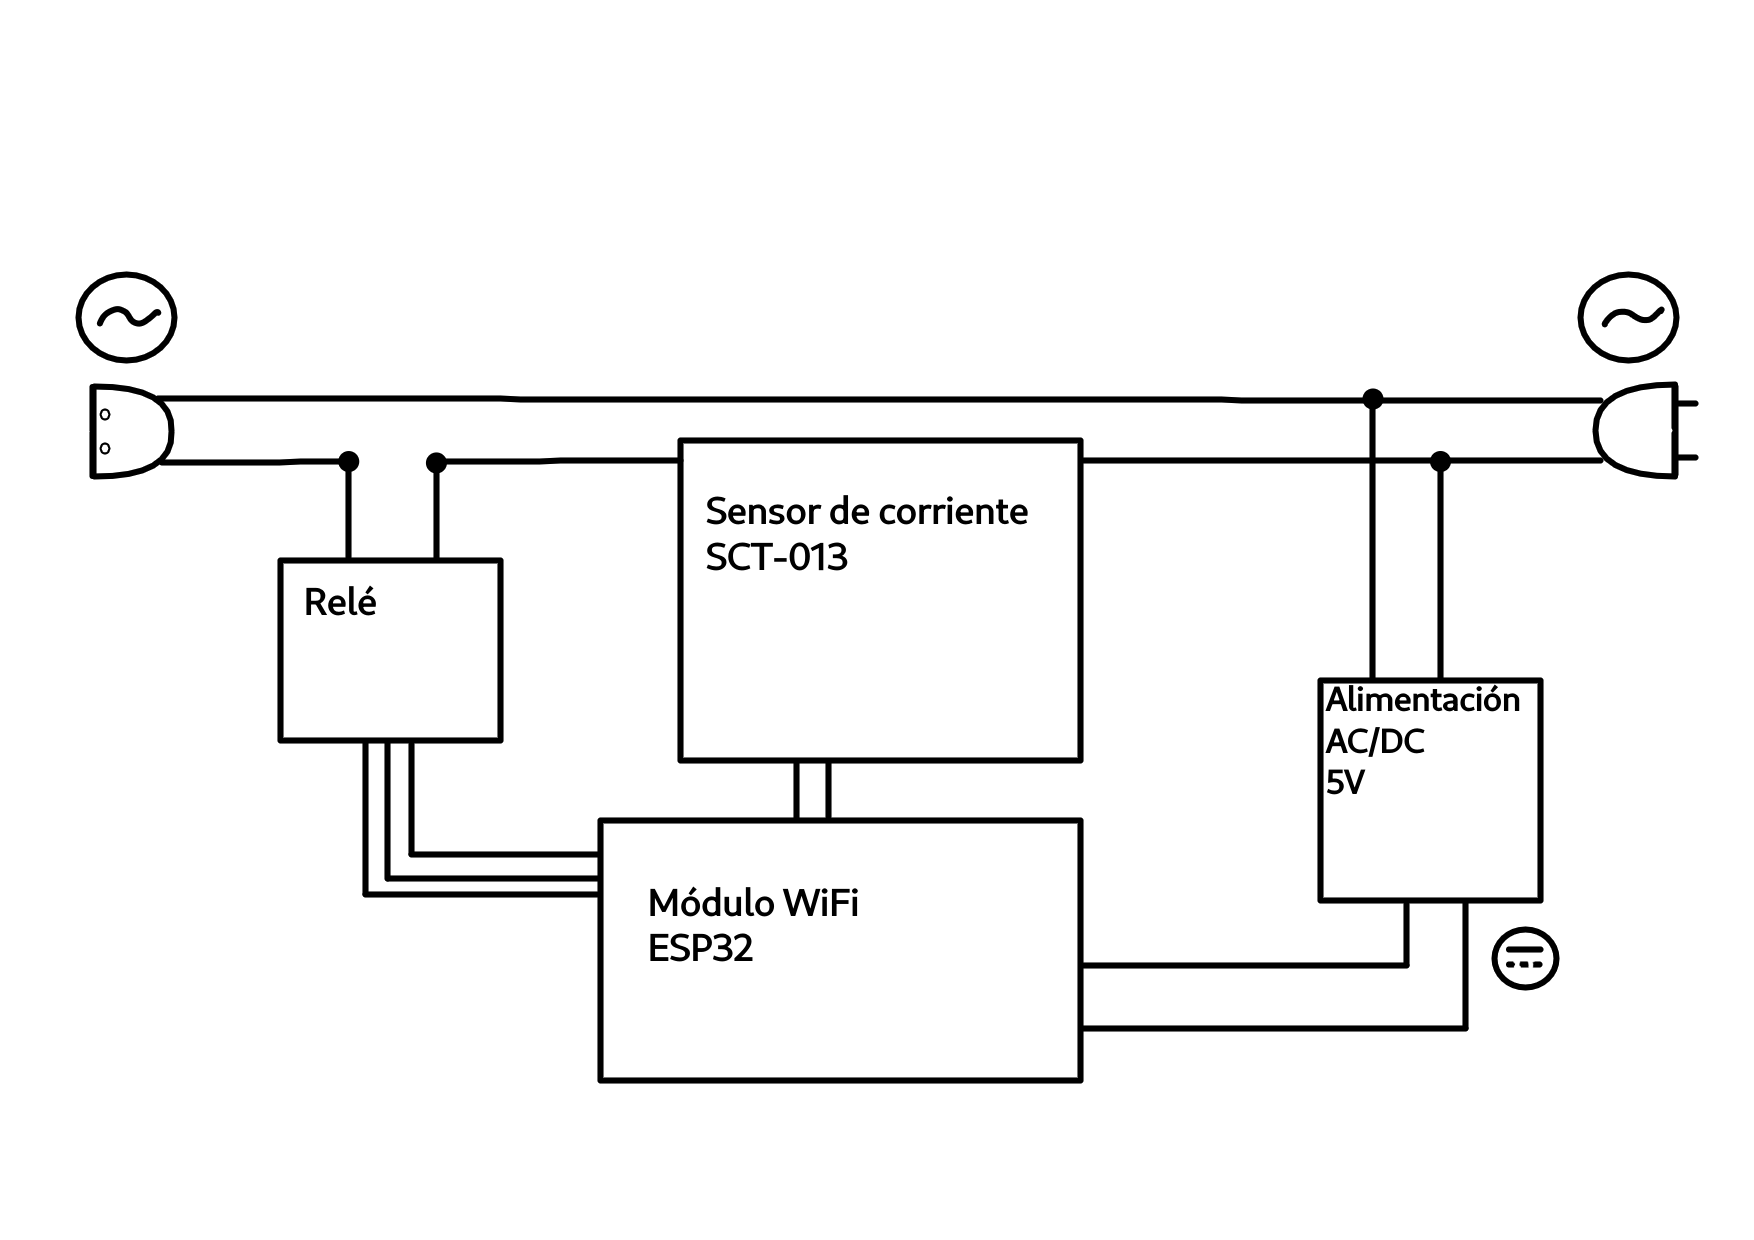
\includegraphics[scale=0.7]{img/esquema_enchufe_inteligente.png}
\end{frame}

\begin{frame}
  \transdissolve[duration=1]
  \frametitle{\insertsubsection}
  Componentes:
  \begin{itemize}
  \item{Sensor de corriente}
  \item{Actuador: Relé}
  \item{Microcontrolador: ESP32}
  \item{Fuente de alimentación}
  \end{itemize}
  % Sensor de corriente: El encargado de realizar las mediciones de
  % consumo
  % Relé: Encargado de encender y apagar el dispositivo conectado
  % según se le indique
  % Microcontrolador: Núcleo del enchufe. Con su programa gestiona el
  % relé, procesa el cálculo del consumo procedente del sensor y
  % envía por wifi esta información al servidor usando MQTT.
  % Fuente de alimentación: Proporciona el voltaje para que opere este subsistema.
\end{frame}

\subsection{Módulo Servidor}
\begin{frame}
  \transdissolve[duration=1]
  \frametitle{\insertsubsection}
  \tableofcontents[currentsection,currentsubsection]
\end{frame}

\begin{frame}
  \transdissolve[duration=1]
  \frametitle{\insertsubsection}
  Componentes:
  \begin{itemize}
  \item{Broker MQTT}
  \item{API}
  \end{itemize}
\end{frame}

\begin{frame}
  \transdissolve[duration=1]
  \frametitle{\insertsubsection}
  \only<1->{Broker MQTT:}

  \uncover<2->{Se escogió Mosquitto. Utiliza un patrón de
    publish-subscribe en temas.}

  \uncover<3->{Cada uno de estos temas representa información de
    consumo de un enchufe o información de control.}

  \uncover<4->{Un programa en el servidor introduce la información de
    consumo en la base de datos.} 
\end{frame}

\begin{frame}
  \transdissolve[duration=1]
  \frametitle{\insertsubsection}
  \only<1->{API:}

  \uncover<2->{Devuelve la información de consumo energético a los
    usuarios finales que lo soliciten mediante peticiones HTTP.}
\end{frame}

\subsection{Módulo App}
\begin{frame}
  \transdissolve[duration=1]
  \frametitle{\insertsubsection}
  \tableofcontents[currentsection,currentsubsection]
\end{frame}

\begin{frame}
  \transdissolve[duration=1]
  \frametitle{\insertsubsection}
  \only<1->{Interfaz simple para consultar la información de consumo
    de los enchufes y manipularlos.}

  \uncover<2->{Funcionalidades:
    \begin{itemize}
    \item{Acceder la información de consumo de cada enchufe}
    \item{Visualizar gráficamente dicha información}
    \item{Controlar el estado de los dispositivos conectados}
    \end{itemize}
  }
  
\end{frame}

\subsection{Pruebas}
\begin{frame}
  \transdissolve[duration=1]
  \frametitle{\insertsubsection}
  \tableofcontents[currentsection,currentsubsection]
\end{frame}

\begin{frame}
  \transdissolve[duration=1]
  \frametitle{\insertsubsection\ Microcontrolador}
  \only<1->{\textbf{Microcontrolador:}

    ¿Cómo realizar pruebas sobre un microcontrolador?}

  \uncover<2->{\textbf{Dificultades:} Tests en un microcontrolador que no tiene
    una interfaz y que depende del correcto funcionamiento de los
    sensores.}

  \uncover<3->{\textbf{Posibilidades:}

    Comunicación por serial o utilizar emuladores (mocking).}
  
  \uncover<4->{Simular los resultados proporcionados por los sensores
    para probar tu propio código.}

  % Escribir tests para tu código en un microcontrolador “sin
  % interfaz” con la que comunicarte puede ser complicado de
  % verificar, además puede costar verificar un programa que depende
  % del correcto funcionamiento de sensores o bibliotecas externas.
  %
  % Para lo primero se puede ejecutar algún programa de test sobre el
  % microcontrolador y analizar la salida por el serial o utilizar
  % algún emulador.
  %
  % Para probar tu código dependiente del de terceros simplemente
  % puedes fijar unos valores y asegurarte de que funcionará
  % debidamente cuando se le proporcionen los valores de entrada
  % esperados.
\end{frame}

\begin{frame}
  \transdissolve[duration=1]
  \frametitle{\insertsubsection\ Servidor}
  \textbf{Server:}

  Usar alguna biblioteca de pruebas y un marco de pruebas para probar
  API y módulo del servidor.
\end{frame}

\begin{frame}
  \transdissolve[duration=1]
  \frametitle{\insertsubsection\ App}
  \textbf{App:}

  Probar la interfaz: Comprobar que los elementos se crean
  correctamente y que el comportamiento al realizar algunas acciones
  es el esperado.

  Se pueden usar bibliotecas genéricas y otras específicas de la
  interfaz para probar su funcionamiento.
\end{frame}

\section{Conclusiones}
\begin{frame}
  \transdissolve[duration=1]
  \frametitle{\insertsection}
  \tableofcontents[currentsection]
\end{frame}

\begin{frame}
  \transdissolve[duration=1]
  \frametitle{\insertsection}
  \begin{itemize}
    \only<1->{\item{\textbf{Accesibilidad:} Este proyecto busca ser una muestra
        de que el Internet de las Cosas es algo que está a nuestro
        alcance.}}
    % Aún comenzando este proyecto sin saber programar en
    % microcontroladores, sin saber soldar, con conocimientos básicos de
    % electrónica y sin experiencia en diseño y programación de
    % interfaces es perfectamente posible alcanzar a crear un proyecto
    % usable e incluso mejorable 
    \uncover<2->{\item{\textbf{Licencia:} El código de este proyecto
        es libre (GPLv3).}}
    % Este sistema siempre puede mejorarse, puede que tal vez a
    % alguien le sirva de base para adaptarlo a sus necesidades y
    % mejorarlo o puede que no, pero la única manera de garantizar
    % esto es mediante una licencia libre
    \uncover<3->{\item{\textbf{Modularidad y usabilidad:} Se puede
        reemplazar algunos de los subsistemas y mantener la
        funcionalidad.}}
    % No es necesario utilizar este mismo enchufe si no se dispone de
    % algún elemento, se puede utilizar otro servidor distinto a una
    % raspberry pi o se puede diseñar una interfaz que se adapte mejor
    % a tus intereses, mientras se comuniquen del mismo modo
    % cualquiera puede llegar, adaptar este proyecto o sustituir
    % alguna pieza y esto gracias al diseño modular y a la licencia
    % del proyecto.
    \uncover<4->{\item{\textbf{Presupuesto asequible:} Con una pequeña
      inversión se puede construir un enchufe inteligente que no
      dependa de terceros.}}
    % El precio puede dar la sensación de crecer en un primer momento,
    % pero muchos de los elementos usados o bien son de uso frecuente
    % en proyectos de electrónica como resistencias, cableado o bien
    % son incluso sustituibles como raspberry pi que también son
    % frecuentes en proyectos informáticos y reutilizables.
  \end{itemize}
\end{frame}

\begin{frame}
  \transdissolve[duration=1]
  \frametitle{Posibles mejoras al sistema}

  Este sistema es una prueba de concepto. Todavía se puede mejorar:

  \begin{itemize}
  \item{Sería más cómodo disponer también de una app móvil.}
    % Procuré utilizar alguna interfaz multiplataforma que no
    % proporcionó resultados esperados, y descarté el prototipado de
    % una aplicación para Android para garantizar una mejor calidad en
    % el resto del sistema
  \item{Disponer de más enchufes podría haber dado lugar a un entorno
    más realista.}
    % Podría haber resultado más interesante para estudiar su uso en
    % entornos más complejos y aprovechar mejor las funcionalidades
    % del sistema, pero la situación actual no ha favorecido esto.
  \item{Se podría haber sacado más provecho de las posibilidades que
    ofrecen las bibliotecas usadas para la interfaz de usuario u
    optimizado la programación del microcontrolador.}
    % Ante la carencia de experiencia se puede mejorar mucho en las
    % buenas prácticas a la hora de programar para Arduino o para la
    % interfaz, si la manera en la que realizar las cosas o sacar
    % partido a las bibliotecas personalizadas de test ha sido la
    % apropiada. A pesar de ello se ha procurado que, dentro de la
    % inexperiencia, todo lo usado estuviera sostenido con una
    % investigación y pruebas.
  \end{itemize}
\end{frame}

\section{Referencias}

\begin{frame}
  \transdissolve[duration=1]
  \frametitle{\insertsubsection}
  \tableofcontents[currentsection]
\end{frame}

\begin{frame}
  \transdissolve[duration=1]
  
  \frametitle{\insertsection}
    
  \footnotesize{
    \begin{thebibliography}{7} % Beamer does not support BibTeX so references must be inserted manually as below
    \bibitem{Repo} Jesús Sánchez de Lechina
      \newblock Código del proyecto
      \newblock \url{https://github.com/jojelupipa/smart-plug}
    \bibitem{Diapositivas} Jesús Sánchez de Lechina
      \newblock Esta presentación
      \newblock \url{https://github.com/jojelupipa/TFG-presentacion}
    \bibitem{Pbaeyens} Pablo Baeyens
      \newblock Guía de uso de beamer
      \newblock \url{https://github.com/dgiim/beamer}
    \bibitem{M42} Mario Román
      \newblock Recopilación de plantillas de Latex.
      \newblock \url{https://github.com/M42/plantillas}
    \end{thebibliography}
  }
\end{frame}

%------------------------------------------------

        \begin{frame}
	\transdissolve[duration=1]

\Huge{\centerline{Fin}}
\end{frame}

%----------------------------------------------------------------------------------------

\end{document}
